\documentclass{beamer}
\usepackage[utf8]{inputenc}
\usepackage[T1]{fontenc}
\usepackage[alf]{abntex2cite}
\usepackage{udesc}
\usepackage{amsfonts,amsmath,amssymb,mathtools}
\usepackage{comment,color, fancybox}
\usepackage{verbatim}
\usepackage{enumitem}
\usepackage{listings}
\usepackage{xcolor}
\usepackage{array}
\usepackage{ragged2e}
\usepackage[ddmmyyyy]{datetime}

\setbeamertemplate{frametitle continuation}{}

\title{Fusão de Imagens em Diferentes Perspectivas para Geração de Fachadas Livres de Oclusão - \citeonline{Maestri2015}}
\subtitle{Trabalho Complementar 1 CGR}
\author{Miguel Alfredo Nunes\\ \texttt{miguel.nunes@edu.udesc.br}}
\date{\today}

\begin{document}

    \begin{frame}
        \titlepage
    \end{frame}
    
    \begin{frame}[allowframebreaks]{Problema}
        
        \begin{itemize}
            \item Privacidade nos serviços de visualização de imagens de ruas - a presença de carros e pedestres que tornam possível identificar pessoas (não necessariamente presentes na imagem) a partir das imagens retirados destes serviços.
            
            \item Google Street View, serviço utilizado no trabalho, já implementa uma funcionalidade de "borramento" de faces e placas de carro, porém isso não é o suficiente.
            
        \end{itemize}
        % \framebreak
        
        % \begin{figure}
        %     \centering
        %     \includegraphics[scale=.35]{exemplo.png}
        %     \caption{Exemplo do problema abordado}
        % \end{figure}
        
    \end{frame}
    
    \begin{frame}{Objetivo}
    
        Objetivo Geral:
        \begin{quote}
            Desenvolver um método eficiente de processamento de imagem que possibilite a remoção de objetos móveis como pessoas e veículos nas imagens de sistemas de visualização de imagens panorâmicas.
        \end{quote}
        
        Objetivos Específicos:
        
        \begin{itemize}[label=\textbullet]
            \item <1-> Criar um método para a remoção de objetos em movimento, em um sistema de imagens de perspectivas diferentes;
            
            \item <2-> Criar um processo para o alinhamento das imagens de diferentes perspectivas;
            
            \item <3-> Criar um processo que identifique os \textit{pixels} referentes ao fundo das imagens, criando uma nova imagem sem oclusão do objetos em movimento;
            
            \item <4-> Verificar a funcionalidade do método testando-o em imagens do GSV e comparando-o com os trabalhos relacionados de acordo com as métricas estabelecidas.
        \end{itemize}
        
    \end{frame}
    
    \begin{frame}{O que foi feito}
        Foi feita uma pesquisa da literatura para determinar o estado da arte na área.
    
        A partir dos trabalhos levantados, foi desenvolvido um algoritmo que identifica objetos que obstruam fachadas de prédios em imagens do Google Street View e as remove, utilizando 3 imagens da mesma fachada, uma vista de frente, uma vista da esquerda e uma vista da direita.
    \end{frame}
    
    \begin{frame}{Recursos/Técnicas Utilizadas}
        \begin{enumerate}[label=({\arabic*})]
            \item <1-> Algoritmo da Distância de Manhatam;
            
            \item <2-> Algoritmo de Identificação de Fundo de \citeonline{Bohm2004};
            
            \item <3-> Método RANSAC (\textit{Random Sample Consensus});
            
            \item <4-> Algoritmo de Transformação de Perspectiva 2D;
            
            \item <5-> Algoritmo de Classificação KNN (\textit{K Nearest Neighbors});
            
            \item <6-> Algoritmo de \textit{Inpainting};
            
            % \item <7-> Métodos de Detecção de Descritores;
            
            \item <7-> Algoritmo SIFT (\textit{Scale Invariant Feature Transform})
            
            \item <8-> Histograma de Gradientes Orientados
            
            \item <9-> \textit{Speeded Up Robust Features} (SURF)
        \end{enumerate}
    \end{frame}
    
    \begin{frame}[allowframebreaks]{Resultados Obtidos}
        O algoritmo desenvolvido teve dificuldades na identificação do fundo das imagens, assim como na identificação de pontos em comum entre as várias perspectivas da mesma fachada, gerando imagens borradas e com artefatos.
        
        \framebreak
        
        \begin{figure}
            \centering
            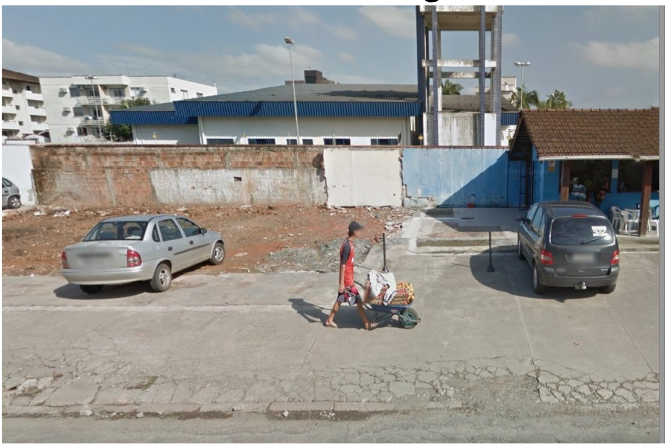
\includegraphics[scale=.4]{exemploE.png}
            \caption{Exemplo de imagem antes do processamento, retirado do artigo}
        \end{figure}
        
        \framebreak
        
        \begin{figure}
            \centering
            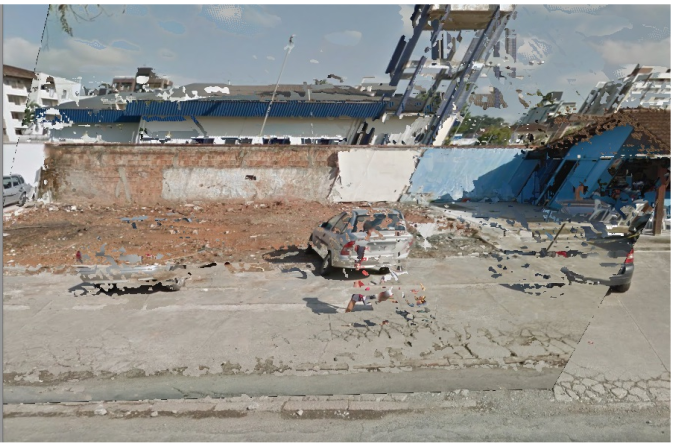
\includegraphics[scale=.4]{exemploD.png}
            \caption{Exemplo de imagem após processamento, retirado do artigo}
        \end{figure}
        
    \end{frame}
    
    \begin{frame}{Conclusão}
        Sistemas como o Google Street View cresceram muito no mundo todo e com eles os problemas de privacidade associados, estes que podem ser resolvidos retirando elementos passíveis de identificação nas imagens do serviço.
        
        \vspace{\baselineskip}
        
        O método desenvolvido no trabalho eliminou a interferência humana na identificação de objetos passíveis a identificação de pessoas, assim como levou um tempo consideravelmente menor que o tempo empregado pelos trabalhos relacionados, porém os resultados obtidos não tiveram a qualidade esperada.
        
        \vspace{\baselineskip}
        
        A causa identificada para a baixa qualidade das imagens resultantes foi o método utilizado para a identificação de fundo.
    \end{frame}
    
    \begin{frame}{Sub-áreas Relacionadas}
        Foi identificado que o trabalho pertence à área de Processamento de Imagens, pois lida com a manipulação de imagens e geração de novas imagens a partir de outras, mas não as gera a partir de dados os modelos computacionais.
    \end{frame}

    \begin{frame}[allowframebreaks]{Referências}
        \bibliography{referencias}
    \end{frame}
    
\end{document}
